% !Rnw weave = knitr
\documentclass[12pt]{article}\usepackage[]{graphicx}\usepackage[]{color}
%% maxwidth is the original width if it is less than linewidth
%% otherwise use linewidth (to make sure the graphics do not exceed the margin)
\makeatletter
\def\maxwidth{ %
  \ifdim\Gin@nat@width>\linewidth
    \linewidth
  \else
    \Gin@nat@width
  \fi
}
\makeatother

\definecolor{fgcolor}{rgb}{0.345, 0.345, 0.345}
\newcommand{\hlnum}[1]{\textcolor[rgb]{0.686,0.059,0.569}{#1}}%
\newcommand{\hlstr}[1]{\textcolor[rgb]{0.192,0.494,0.8}{#1}}%
\newcommand{\hlcom}[1]{\textcolor[rgb]{0.678,0.584,0.686}{\textit{#1}}}%
\newcommand{\hlopt}[1]{\textcolor[rgb]{0,0,0}{#1}}%
\newcommand{\hlstd}[1]{\textcolor[rgb]{0.345,0.345,0.345}{#1}}%
\newcommand{\hlkwa}[1]{\textcolor[rgb]{0.161,0.373,0.58}{\textbf{#1}}}%
\newcommand{\hlkwb}[1]{\textcolor[rgb]{0.69,0.353,0.396}{#1}}%
\newcommand{\hlkwc}[1]{\textcolor[rgb]{0.333,0.667,0.333}{#1}}%
\newcommand{\hlkwd}[1]{\textcolor[rgb]{0.737,0.353,0.396}{\textbf{#1}}}%
\let\hlipl\hlkwb

\usepackage{framed}
\makeatletter
\newenvironment{kframe}{%
 \def\at@end@of@kframe{}%
 \ifinner\ifhmode%
  \def\at@end@of@kframe{\end{minipage}}%
  \begin{minipage}{\columnwidth}%
 \fi\fi%
 \def\FrameCommand##1{\hskip\@totalleftmargin \hskip-\fboxsep
 \colorbox{shadecolor}{##1}\hskip-\fboxsep
     % There is no \\@totalrightmargin, so:
     \hskip-\linewidth \hskip-\@totalleftmargin \hskip\columnwidth}%
 \MakeFramed {\advance\hsize-\width
   \@totalleftmargin\z@ \linewidth\hsize
   \@setminipage}}%
 {\par\unskip\endMakeFramed%
 \at@end@of@kframe}
\makeatother

\definecolor{shadecolor}{rgb}{.97, .97, .97}
\definecolor{messagecolor}{rgb}{0, 0, 0}
\definecolor{warningcolor}{rgb}{1, 0, 1}
\definecolor{errorcolor}{rgb}{1, 0, 0}
\newenvironment{knitrout}{}{} % an empty environment to be redefined in TeX

\usepackage{alltt}
\usepackage[backend=biber, sorting=nyt, maxcitenames=2, doi=false,url=false, style=apa]{biblatex} 
\bibliography{/Users/Owner/Documents/Tex/all,/Users/Owner/Documents/Thesis/thesis_ref}
\DeclareLanguageMapping{american}{american-apa}
\usepackage{xr}
\externaldocument{Eyster_germ_ms}
\renewcommand{\thetable}{S\arabic{table}} 
\renewcommand{\thefigure}{S\arabic{figure}}
\usepackage{graphicx}
\graphicspath{}
\usepackage{caption}
\usepackage{subcaption}
\captionsetup[subfigure]{position=top}
\usepackage[figuresleft]{rotating}
\usepackage{longtable}
\usepackage[margin=.5in]{geometry}
\usepackage{float}
\usepackage{makecell}

\title{\textbf{Supporting information for:}  \\ \bigskip Invader success and changing climate: Comparisons in the native and introduced range of seven plant species}\author{Harold N. Eyster* \&  Elizabeth Wolkovich}
\date{*Corresponding author. Please direct any questions or comments to haroldeyster@gmail.com. }


  




\IfFileExists{upquote.sty}{\usepackage{upquote}}{}
\begin{document}
\maketitle
\tableofcontents
\section{Additional methods}
\subsection{Defining Invasive Species}
	There is no consensus on how to classify a species as invasive \parencite{Colautti2004}. The most common terms include `exotic,' `introduced,' `naturalized,' `nonindigenous,' `established,' `alien,' `noxious,' `weedy,' and `invasive.' These terms can be grouped into those that describe the provenance of the species (e.g., exotic, introduced, alien, non-indigenous), those that describe its ability to grow and compete in the new ecosystem (e.g., naturalized, established), and those that describe its impact on the receiving ecosystem (e.g., noxious, weedy, harmful). The International Union for the Conservation of Nature (IUCN, 2008) describes invasive species as: ``organisms introduced by man [sic] into places out of their natural range of distribution, where they become established and disperse, generating a negative impact." \nocite{IUCN2008is} However, this definition contains three subjective elements: what timepoint of a species' range is `natural,' whether humans are a natural part of nature, and what is defined as a negative impact \parencite{Munro2019}. To both acknowledge and allay some of these subjective elements, this paper will follow Richardson et al.'s \parencite{Richardson2000,Richardson2011} definition of invasive species. Invasive species are thus those that (1) are introduced across a previously unpenetrated barrier, (2) successfully reproduce in the place of introduction to create a stable local population, and finally (3) spread to produce fit offspring a substantial distance from the place of introduction.

\subsection{Study species details}
\textit{Capsella bursa-pastoris} (CAPBUR; Shepard's Purse) is an annual or biennial herbaceous plant in Brassicaceae. It grows 10 to 80 cm tall, typically blooming in late spring \parencite{Defelice2001}. It originated in Europe, and was introduced to the New World as a medicinal herb---it is now found across Canada, the US, and Mexico \parencite{Westrich1989}.
	
	\textit{Chelidonium majus} (CHEMAJ; Greater Celandine) is an herbaceous biennial member of Papaveraceae. It is native to Eurasia and North Africa and was introduced to the US by the 1670s as a medicinal. It is now found across the Eastern US and Canada and portions of the west \parencite{Holm1979}. 
	
	\textit{Dactylis glomerata} (DACGLO; Orchard Grass) is a cool-season, perennial grass (Poaceae). Plants grow up to 120 cm tall and have roots up to 60 cm long \parencite{Moser1996}. This plant originated in central and western Europe, and was intentionally introduced into the US in the 1750s \parencite{Bush2012} as a forage grass for pasture and hay \parencite{Ogle2011}.  
	
	\textit{Plantago lanceolata} (PLALAN; Narrow-leaved Plantain) is a perennial member of  Plantaginaceae. It has narrow, ribbed leaves and grows to 1m tall. It is native to Eurasia, and has successfully colonized the world's mid-latitudes \parencite{Holm1977}.
	
	\textit{Plantago major} (PLAMAJ; Broad-leaved Plantain) is a perennial member of Plantaginaceae. It has broad, smooth leaves, and grows to 15cm tall. Native to Europe, it was introduced into North America for its medicinal uses \parencite{Knobloch1996,Samuelsen2000}.
	
	\textit{Rumex crispus} (RUMCRI; Curly Dock) is a perennial herbaceous plant in Polygonaceae, and grows to 160 cm. It is native to Europe, Asia, and Africa, and was introduced for its medicinal uses into North America where it now found across much of the continent \parencite{USDA2010}. 
	
	\textit{Taraxacum officinale} (TAROFF; Dandelion) is a perennial herbaceous plant in the Asteraceae family, and grows to 60 cm. It is native to Eurasia, but is now found in all 50 US states, much of Canada, and Mexico \parencite{USDA1971}.

\subsection{Sampling details}

	\begin{center}
		\begin{table}[H]
			\centering
			\caption {Total number of seed-producing individuals and populations from which seeds were collected.} \label{tab:seeds}  
			\begin{tabular}{c|c|c|c}
				\makecell{\textbf{US} \\ \textbf{populations}} & \makecell{\textbf{US} \\  \textbf{individuals}} & \makecell{\textbf{European} \\ \textbf{populations}} & \makecell{\textbf{European} \\ \textbf{individuals}} \\
				\hline
				3&	21&	13&	63\\
			\end{tabular}
		\end{table}
	\end{center}
\subsection{Period/light luminance}
Some species have sufficient Pfr (the active form of phytochrome pigment, often necessary to induce germination) and so do not need any light to break dormancy, others just need a pulse of red light to break dormancy (the red light converts the inactive phytochrome into Pfr) \parencite{Casal998}.  Other species, including \textit{Plantago major}, take much longer to build up the requisite Pfr, and so have much higher germination success when exposed to longer periods of light (with nearly 100\% germination after 48 hours of exposure for \textit{P. major}) \parencite{Pons1991}. Finally, some species have a high irradiance response (HIR), germinating poorly when exposed to high luminance light or prolonged light \parencite{Roberts1987}. Beyond interspecific variation, there is also intraspecific variation in the relationship between dormancy and light \parencite{Probert1986}. Across all populations, germination rate seems to be log-normally related to photon dosage \parencite{Ellis1986}. Light may begin inhibiting germination for HIR species at about 0.1 mol/m\textsuperscript{2}/day--1 mol/m\textsuperscript{2}/day \parencite{Baskin1998,Ellis1986}, while other species peak above 10 mol/m\textsuperscript{2}/day \parencite{Ellis1986}. The differing levels of light necessary to break dormancy means that any chosen light regime will be better for some species and worse for others. 
	
	The goal of these experiments is to create germination rates that are sufficient to observe variation in responses to treatments. Thus, we chose an intermediate light exposure at which all of the species should germinate at substantial levels, but which may not be ideal for any species. In selecting how much light to use, this experiment erred on the side of too much light rather than not enough, since at least one of our species is known to need large amounts of light (\textit{Plantago major}---\textcite{Pons1991}), and none are known to exhibit HIR (although a \textit{D. glomerata} subspecies in southern Europe does exhibit HIR \parencite{Probert1986}, but this subspecies is not thought to have been collected for this study). Thus this experiment used a length of eight hours at a luminance of 75 micromol/m\textsuperscript{2}/second to yield a daily photon dosage of 2.16 mol/m\textsuperscript{2}. \textcite{Baskin1998} recommend that the light period coincide with the high-temperature period. Thus, this experiment exposed the seeds to eight hours of fluorescent light during the high-temperature thermoperiod. 
	
\subsection{Substrate and planting depth:} \textcite{Popay1970} show that \textit{C. bursa-pastoris} seeds germinated about equally on filter paper as on top of soil, but showed much decreased germination when inserted into soil. The effects of planting substrate and depth have not been studied in most of the study species. However, a study on a species related to \textit{D. glomerata} suggests that \textit{D. glomerata} may germinate better in soil \parencite{Andrews1974}. Additionally, a difference in depth of just a couple millimeters can result in extreme differences in light availability \parencite{Tester1987}. Thus each seed was placed on top of Fafard Growing Mix (a mixture of fine peat moss, fine perlite, and vermiculite) soil, with each seed in its own individual tray cell.
\printbibliography()
\section{Raw Data Plots}

\begin{figure}[H]
  \centering
  \subcaptionbox{CAPBUR\label{fig:grCAPBUR}}
  {\includegraphics[scale=.5, page=7, trim=0cm 0cm 3cm 1.2cm, clip=TRUE]{supplement.pdf}}
  \subcaptionbox{CHEMAJ\label{fig:grCHEMAJ}}
  {\includegraphics[scale=.5, page=3, trim=0cm 0cm 3cm 1.2cm, clip=TRUE]{supplement.pdf}}
  \subcaptionbox{DACGLO\label{fig:grDACGLO}}
  {\includegraphics[scale=.5, page=6, trim=0cm 0cm 3cm 1.2cm, clip=TRUE]{supplement.pdf}}
  \subcaptionbox{PLALAN\label{fig:grPLALAN}}
  {\includegraphics[scale=.5, page=2, trim=0cm 0cm 3cm 1.2cm, clip=TRUE]{supplement.pdf}}
\end{figure}
\begin{figure}[H]\ContinuedFloat
  \centering
  \subcaptionbox{PLAMAJ\label{fig:grPLAMAJ}}
  {\includegraphics[scale=.5, page=1, trim=0cm 0cm 3cm 1.2cm, clip=TRUE]{supplement.pdf}}
  \subcaptionbox{RUMCRI\label{fig:grRUMCRI}}
  {\includegraphics[scale=.5, page=4, trim=0cm 0cm 3cm 1.2cm, clip=TRUE]{supplement.pdf}}
  \subcaptionbox{TAROFF\label{fig:grTAROFF}}
  {\includegraphics[scale=.5, page=5, trim=0cm 0cm 0cm 1.2cm, clip=TRUE]{supplement.pdf}}
  \caption{Height vs. age by stratification and temperature. Growth rate can be approximately linear.  Pink represents European   plants, while blue represents those from  North America \label{fig:lmgr}}
\end{figure}

\begin{figure}[H]
  \centering
  \includegraphics[scale=.9]{figure5} 
  \caption{Unmodeled germination rate by population origin, and across stratification length and temperature treatments for each species (mean +/- standard error). Note the variable y-axis scale.} \label{fig:rawrate}
\end{figure}

\begin{figure}[H]
  \centering
  \includegraphics[scale=.9]{figure7} 
  \caption{Unmodeled germination timing by population origin, and across stratification length and temperature treatments for   each species (mean +/- standard error). Note the variable y-axis scale.} \label{fig:rawtime} 
\end{figure}
\begin{figure}[H]
  \centering
  \includegraphics[scale=.9]{figure9} 
  \caption{Unmodeled growth rate by population origin, and across stratification length and temperature treatments for each   species (mean +/- standard error). Note the variable y-axis scale.} \label{fig:rawgrowth} 
\end{figure}

\section{Model Results}
\subsection{Coefficient tables}


% latex table generated in R 3.5.1 by xtable 1.8-3 package
% Wed Apr 15 21:39:27 2020
\begin{longtable}{rrrrrrr}
\caption{Summary of multilevel model of germination rate. Output is in logit(fraction germinated)} \\ 
  & mean & sd & 2.5\% & 50\% & 97.5\% & Rhat \\ 
  \hline
(Intercept) & 1.82 & 0.48 & 0.93 & 1.80 & 2.79 & 1.00 \\ 
  origin & -0.10 & 0.72 & -1.50 & -0.09 & 1.33 & 1.00 \\ 
  strat & 0.17 & 0.68 & -1.11 & 0.14 & 1.65 & 1.00 \\ 
  temp1 & 0.20 & 0.54 & -0.78 & 0.17 & 1.31 & 1.00 \\ 
  temp2 & -0.10 & 0.45 & -0.95 & -0.11 & 0.82 & 1.00 \\ 
  temp3 & -0.18 & 0.43 & -1.03 & -0.18 & 0.68 & 1.00 \\ 
  origin $\times$ strat & -0.01 & 0.84 & -1.63 & -0.03 & 1.72 & 1.00 \\ 
  origin $\times$ temp1 & -0.41 & 0.71 & -1.78 & -0.42 & 0.97 & 1.00 \\ 
  origin $\times$ temp2 & 0.76 & 0.85 & -0.82 & 0.74 & 2.50 & 1.00 \\ 
  origin $\times$ temp3 & 0.88 & 0.75 & -0.54 & 0.87 & 2.36 & 1.00 \\ 
  strat $\times$ temp1 & 0.61 & 0.73 & -0.85 & 0.60 & 2.05 & 1.00 \\ 
  strat $\times$ temp2 & 0.45 & 0.71 & -0.86 & 0.41 & 1.98 & 1.00 \\ 
  strat $\times$ temp3 & 0.59 & 0.76 & -0.82 & 0.55 & 2.22 & 1.00 \\ 
  origin $\times$ strat $\times$ temp1 & 0.53 & 1.09 & -1.59 & 0.52 & 2.72 & 1.00 \\ 
  origin $\times$ strat $\times$ temp2 & 0.11 & 1.00 & -1.82 & 0.11 & 2.11 & 1.00 \\ 
  origin $\times$ strat $\times$ temp3 & 0.80 & 1.36 & -1.65 & 0.73 & 3.63 & 1.00 \\ 
  \hline
\label{tab:mod_rate}
\end{longtable}
% latex table generated in R 3.5.1 by xtable 1.8-3 package
% Wed Apr 15 21:39:27 2020
\begin{longtable}{rrrrrrr}
\caption{Summary of multilevel model of germination timing. Output is in log(days)} \\ 
  & mean & sd & 2.5\% & 50\% & 97.5\% & Rhat \\ 
  \hline
(Intercept) & 2.75 & 0.25 & 2.28 & 2.75 & 3.26 & 1.00 \\ 
  origin & -0.15 & 0.17 & -0.48 & -0.15 & 0.21 & 1.00 \\ 
  strat & -0.11 & 0.19 & -0.50 & -0.10 & 0.22 & 1.00 \\ 
  temp1 & -0.37 & 0.11 & -0.58 & -0.37 & -0.13 & 1.00 \\ 
  temp2 & -0.47 & 0.16 & -0.75 & -0.47 & -0.14 & 1.00 \\ 
  temp3 & -0.36 & 0.14 & -0.62 & -0.37 & -0.07 & 1.00 \\ 
  origin $\times$ strat & 0.16 & 0.20 & -0.22 & 0.16 & 0.56 & 1.00 \\ 
  origin $\times$ temp1 & 0.06 & 0.18 & -0.29 & 0.06 & 0.41 & 1.00 \\ 
  origin $\times$ temp2 & 0.05 & 0.24 & -0.43 & 0.05 & 0.49 & 1.00 \\ 
  origin $\times$ temp3 & -0.21 & 0.19 & -0.59 & -0.21 & 0.16 & 1.00 \\ 
  strat $\times$ temp1 & 0.05 & 0.19 & -0.32 & 0.05 & 0.46 & 1.00 \\ 
  strat $\times$ temp2 & -0.09 & 0.20 & -0.48 & -0.09 & 0.33 & 1.00 \\ 
  strat $\times$ temp3 & -0.23 & 0.16 & -0.53 & -0.24 & 0.11 & 1.00 \\ 
  origin $\times$ strat $\times$ temp1 & 0.01 & 0.24 & -0.49 & 0.01 & 0.48 & 1.00 \\ 
  origin $\times$ strat $\times$ temp2 & -0.07 & 0.34 & -0.77 & -0.06 & 0.59 & 1.00 \\ 
  origin $\times$ strat $\times$ temp3 & 0.57 & 0.26 & 0.05 & 0.58 & 1.06 & 1.00 \\ 
  \hline
\label{tab:mod_time}
\end{longtable}
% latex table generated in R 3.5.1 by xtable 1.8-3 package
% Wed Apr 15 21:39:27 2020
\begin{longtable}{rrrrrrr}
\caption{Summary of multilevel model of growth rate.  Output is in cm/day} \\ 
  & mean & sd & 2.5\% & 50\% & 97.5\% & Rhat \\ 
  \hline
(Intercept) & 0.16 & 0.05 & 0.07 & 0.16 & 0.25 & 1.00 \\ 
  origin & 0.01 & 0.01 & -0.02 & 0.01 & 0.03 & 1.00 \\ 
  strat & 0.01 & 0.01 & -0.01 & 0.01 & 0.02 & 1.00 \\ 
  temp1 & -0.02 & 0.01 & -0.04 & -0.02 & 0.01 & 1.00 \\ 
  temp2 & -0.04 & 0.01 & -0.07 & -0.04 & -0.02 & 1.00 \\ 
  temp3 & -0.04 & 0.02 & -0.08 & -0.04 & -0.01 & 1.00 \\ 
  origin $\times$ strat & -0.01 & 0.01 & -0.03 & -0.01 & 0.02 & 1.00 \\ 
  origin $\times$ temp1 & 0.01 & 0.01 & -0.02 & 0.01 & 0.03 & 1.00 \\ 
  origin $\times$ temp2 & -0.02 & 0.02 & -0.05 & -0.02 & 0.01 & 1.00 \\ 
  origin $\times$ temp3 & -0.03 & 0.02 & -0.06 & -0.03 & 0.01 & 1.00 \\ 
  strat $\times$ temp1 & -0.00 & 0.01 & -0.03 & -0.00 & 0.02 & 1.00 \\ 
  strat $\times$ temp2 & -0.06 & 0.02 & -0.11 & -0.06 & -0.03 & 1.00 \\ 
  strat $\times$ temp3 & -0.06 & 0.02 & -0.11 & -0.06 & -0.02 & 1.00 \\ 
  origin $\times$ strat $\times$ temp1 & 0.01 & 0.02 & -0.03 & 0.01 & 0.04 & 1.00 \\ 
  origin $\times$ strat $\times$ temp2 & 0.07 & 0.03 & 0.02 & 0.07 & 0.13 & 1.00 \\ 
  origin $\times$ strat $\times$ temp3 & 0.04 & 0.02 & -0.01 & 0.04 & 0.09 & 1.00 \\ 
  \hline
\label{tab:mod_gr}
\end{longtable}




\subsection{Inter-population variability}
\pagebreak
\begin{figure}[H]
\centering
\fbox{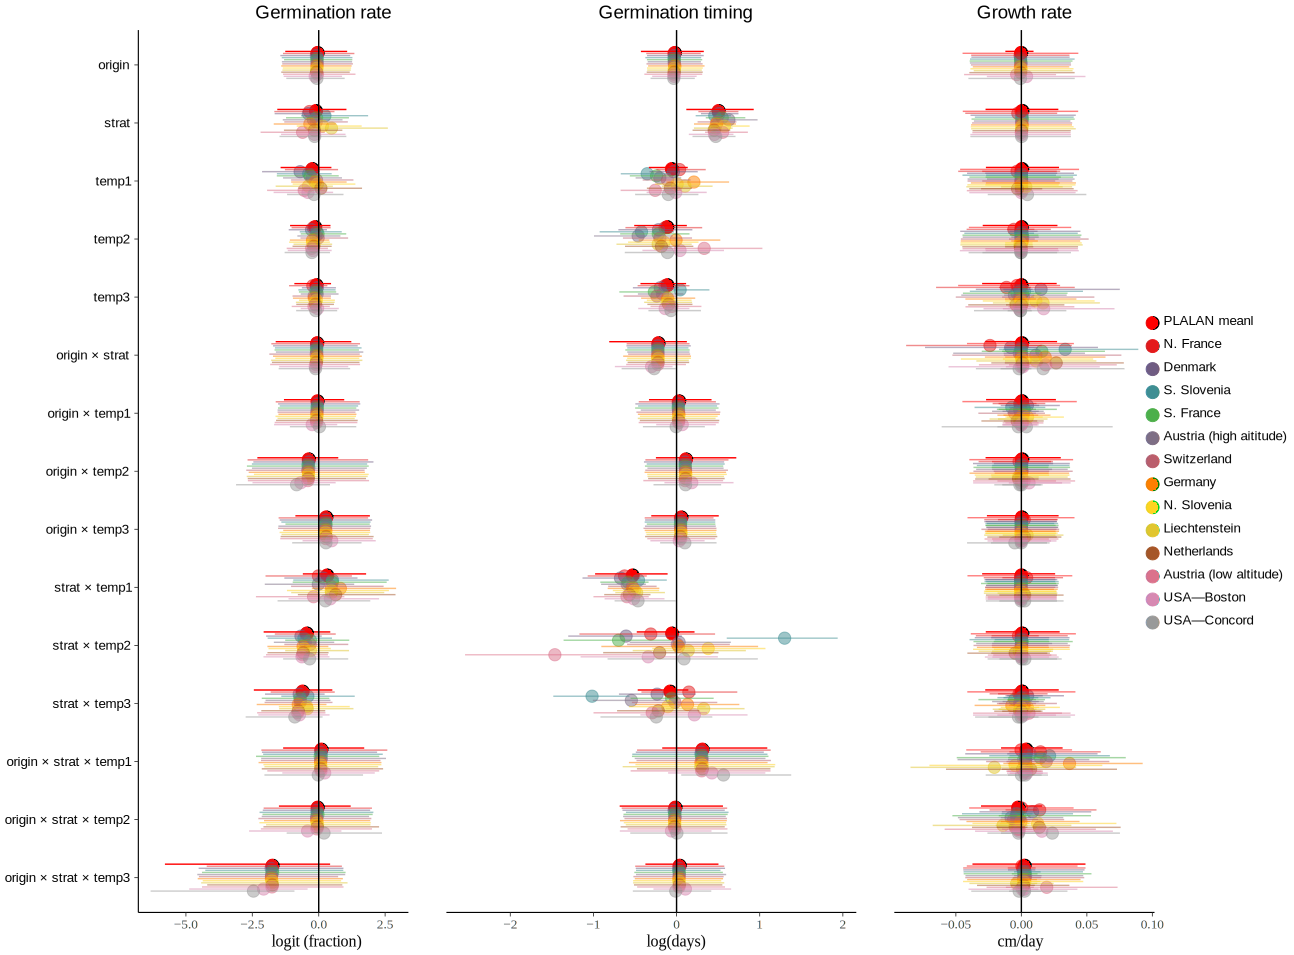
\includegraphics[scale=.67,angle=-90]{PLALAN_pops_plot.pdf}}
\caption{Germinatio rate, germination timing, and growth rate multilevel model coefficients with 95\% credible intervals for PLALAN (\textit{Plantago Lanceolata}), showing main random effect of PLALAN, and random effects of each population. Zero represents the global mean fixed effect across all species. Intercept coefficients not shown.}
\label{fig:pops}
\end{figure}
\end{document}
